\pdfminorversion=5
\documentclass[unnumsec,webpdf,contemporary,large]{oup-authoring-template}

\usepackage{graphicx}
\usepackage{amsmath}
\usepackage{url}
\usepackage{booktabs}

\graphicspath{{figures/}}

% The CTAN bundle does not include the optional PNAS society logo referenced by the class.
\makeatletter
\def\societylogo{}
\makeatother

\begin{document}

\journaltitle{Bioinformatics}
\DOI{DOI added during production}
\copyrightyear{2026}
\pubyear{2026}
\vol{XX}
\issue{x}
\access{Published: Date added during production}
\appnotes{Application Note}
\firstpage{1}

\title[CellChatAccelRcpp]{CellChatAccelRcpp: scalable Rcpp acceleration of CellChat inference for large single-cell communication analyses}

\author[1,$\ast$]{Zifeng Deng}

\address[1]{\orgname{Hainan Bielefeld University of Applied Sciences}, \orgaddress{\state{Hainan}, \country{China}}}

\corresp[$\ast$]{Corresponding author. \href{mailto:zifengd8@gmail.com}{zifengd8@gmail.com}}

\received{Date}{0}{2026}
\revised{Date}{0}{2026}
\accepted{Date}{0}{2026}

\abstract{
\textbf{Summary:}
CellChat is widely used to infer cell-cell communication from single-cell transcriptomic data, but repeated communication probability estimation becomes a computational bottleneck as studies move from individual samples to large atlases and benchmark cohorts.
We present CellChatAccelRcpp, an R/Rcpp acceleration layer that preserves the standard CellChat object interface while replacing selected runtime-critical routines with compiled implementations.
The package accelerates triMean-based expression aggregation, ligand-receptor communication probability estimation, pathway-level probability aggregation and network aggregation without changing the downstream CellChat workflow.
Across 12 real single-cell datasets, six target cell scales and three random repeats, CellChatAccelRcpp achieved an overall median 11.4-fold speedup over the original CellChat workflow.
Median elapsed time decreased from 426.6 s to 36.0 s in 216 paired original/accelerated comparisons.
The accelerated outputs were numerically matched to CellChat, with a maximum absolute probability difference of $1.39 \times 10^{-16}$ and a minimum Pearson correlation of 1.000 across all paired comparisons.
\\
\textbf{Availability and implementation:}
CellChatAccelRcpp is implemented in R and C++ via Rcpp and released under GPL-3 at \url{https://github.com/Blake-Deng/CellChatAccelRcpp}.
The repository contains source code, installation instructions, reproducible benchmark scripts, processed benchmark tables, Supplementary Table S1 and figure-generation scripts.
\\
\textbf{Contact:}
\href{mailto:zifengd8@gmail.com}{zifengd8@gmail.com}
\\
\textbf{Supplementary information:}
Supplementary data are available in the project repository and in the submission package.
}

\keywords{single-cell RNA-seq, cell-cell communication, CellChat, Rcpp, computational acceleration}

\maketitle

\section{Introduction}

Single-cell RNA sequencing has made it possible to describe cellular states across tissues, diseases and perturbations at atlas scale \citep{hao2021integrated}.
After cell annotation, cell-cell communication analysis is commonly used to convert these cellular maps into hypotheses about ligand-receptor signaling among cell groups.
CellChat provides a widely adopted R framework for inferring and interpreting communication networks from single-cell expression data \citep{jin2021cellchat}.
Its object model, curated interaction database and visualization ecosystem make it attractive for routine biological analysis, but the probability estimation and aggregation steps can become expensive when users run large samples, repeated subsampling experiments or benchmark cohorts.

CellChatAccelRcpp addresses this practical scaling problem by accelerating selected CellChat hot paths while preserving the original biological model and user-facing workflow.
The goal is not to introduce a new communication score, but to provide compiled implementations that return CellChat-compatible probability tensors and network summaries.
This design allows users to scale existing CellChat analyses and still compare outputs directly with prior CellChat results.

\section{Materials and methods}

\subsection{Implementation}

CellChatAccelRcpp is an R package with C++ kernels exposed through Rcpp \citep{eddelbuettel2011rcpp}.
The current implementation accelerates group-level average expression under the triMean setting, ligand-receptor communication probability computation, pathway-level probability aggregation and final network aggregation.
Its exported probability, pathway and network functions operate on standard CellChat objects and return objects with the same downstream fields used by CellChat visualization and network analysis functions.

The package currently targets single-dataset RNA-based CellChat workflows using \texttt{type = "triMean"} and \texttt{population.size = FALSE}.
It does not yet validate spatial distance constraints, merged CellChat objects, alternative averaging functions or full CellChat v2 workflows.
For new CellChat settings, the repository provides an equivalence-check script that compares accelerated and original outputs on a representative object before running larger batches.

\subsection{Benchmark design}

We benchmarked CellChatAccelRcpp against the original CellChat workflow on 12 real single-cell datasets stored in the benchmark workspace, including datasets from the \texttt{3CA\_data} and \texttt{normal\_control} collections.
Each dataset was evaluated at six target cell scales: 1k, 5k, 10k, 25k, 50k and all available cells.
For every dataset-scale pair, three random repeats were run from the same prepared CellChat object, creating 216 paired original/accelerated full-workflow comparisons.
Additional ablation runs disabled the accelerated probability kernel, pathway aggregation or network aggregation to estimate the contribution of each component.

Experiments were run in a conda-managed R environment on a Linux server with 256 CPU threads and approximately 1 TiB RAM.
The benchmark runner used checkpointing at the prepared-object and computed-result levels, so interrupted large-scale runs could resume without recomputing completed stages.
Runtime was measured as elapsed wall-clock time for each engine-specific inference run.
Speedup was calculated as original CellChat runtime divided by CellChatAccelRcpp runtime.
Numerical equivalence was assessed by flattening the CellChat communication probability tensor and calculating the maximum absolute difference and Pearson correlation between the original and accelerated outputs.

\section{Results}

CellChatAccelRcpp completed the benchmark without failed metric records.
The final benchmark comprised 216 paired original/accelerated full-workflow comparisons and 648 component-ablation runs, yielding 1296 successful metric rows.
Across paired full-workflow comparisons, the original CellChat median runtime was 426.6 s, whereas CellChatAccelRcpp completed the same inference steps in a median of 36.0 s, corresponding to an overall median speedup of 11.4-fold (Figure~\ref{fig:main}).

The speedup was consistent across cell scales.
Median speedup was 37.4-fold at 1k cells, 15.3-fold at 5k cells, 11.0-fold at 10k cells, 8.0-fold at 25k cells, 6.0-fold at 50k cells and 6.0-fold when using all available cells.
The smaller fold change at the largest scales reflects fixed overheads and non-accelerated CellChat steps becoming a larger fraction of the full workflow after the probability kernel is optimized.
Nevertheless, the accelerated workflow reduced large-scale runs from several minutes to roughly one minute in the median case.

Acceleration did not alter the inferred communication probabilities beyond floating-point precision.
Across all 216 paired comparisons, the maximum absolute probability difference was $1.39 \times 10^{-16}$ and the minimum Pearson correlation between original and accelerated probability tensors was 1.000.
These results support drop-in use of CellChatAccelRcpp when users need CellChat-compatible outputs rather than a different scoring model.

The ablation analysis identified the communication probability kernel as the dominant source of performance gain.
Disabling the accelerated kernel increased runtime by a median 11.35-fold relative to the full accelerated path, whereas disabling pathway aggregation produced a median 1.04-fold slowdown and disabling network aggregation produced a median 1.00-fold change.
Together, the benchmark and ablation results show that CellChatAccelRcpp accelerates the dominant CellChat inference bottleneck while preserving the probability tensors used for downstream biological interpretation.
The major practical benefit comes from replacing the repeated ligand-receptor probability calculation with compiled code, while the additional aggregation kernels provide smaller but useful reductions in batch analyses.

\begin{figure*}[t]
\centering
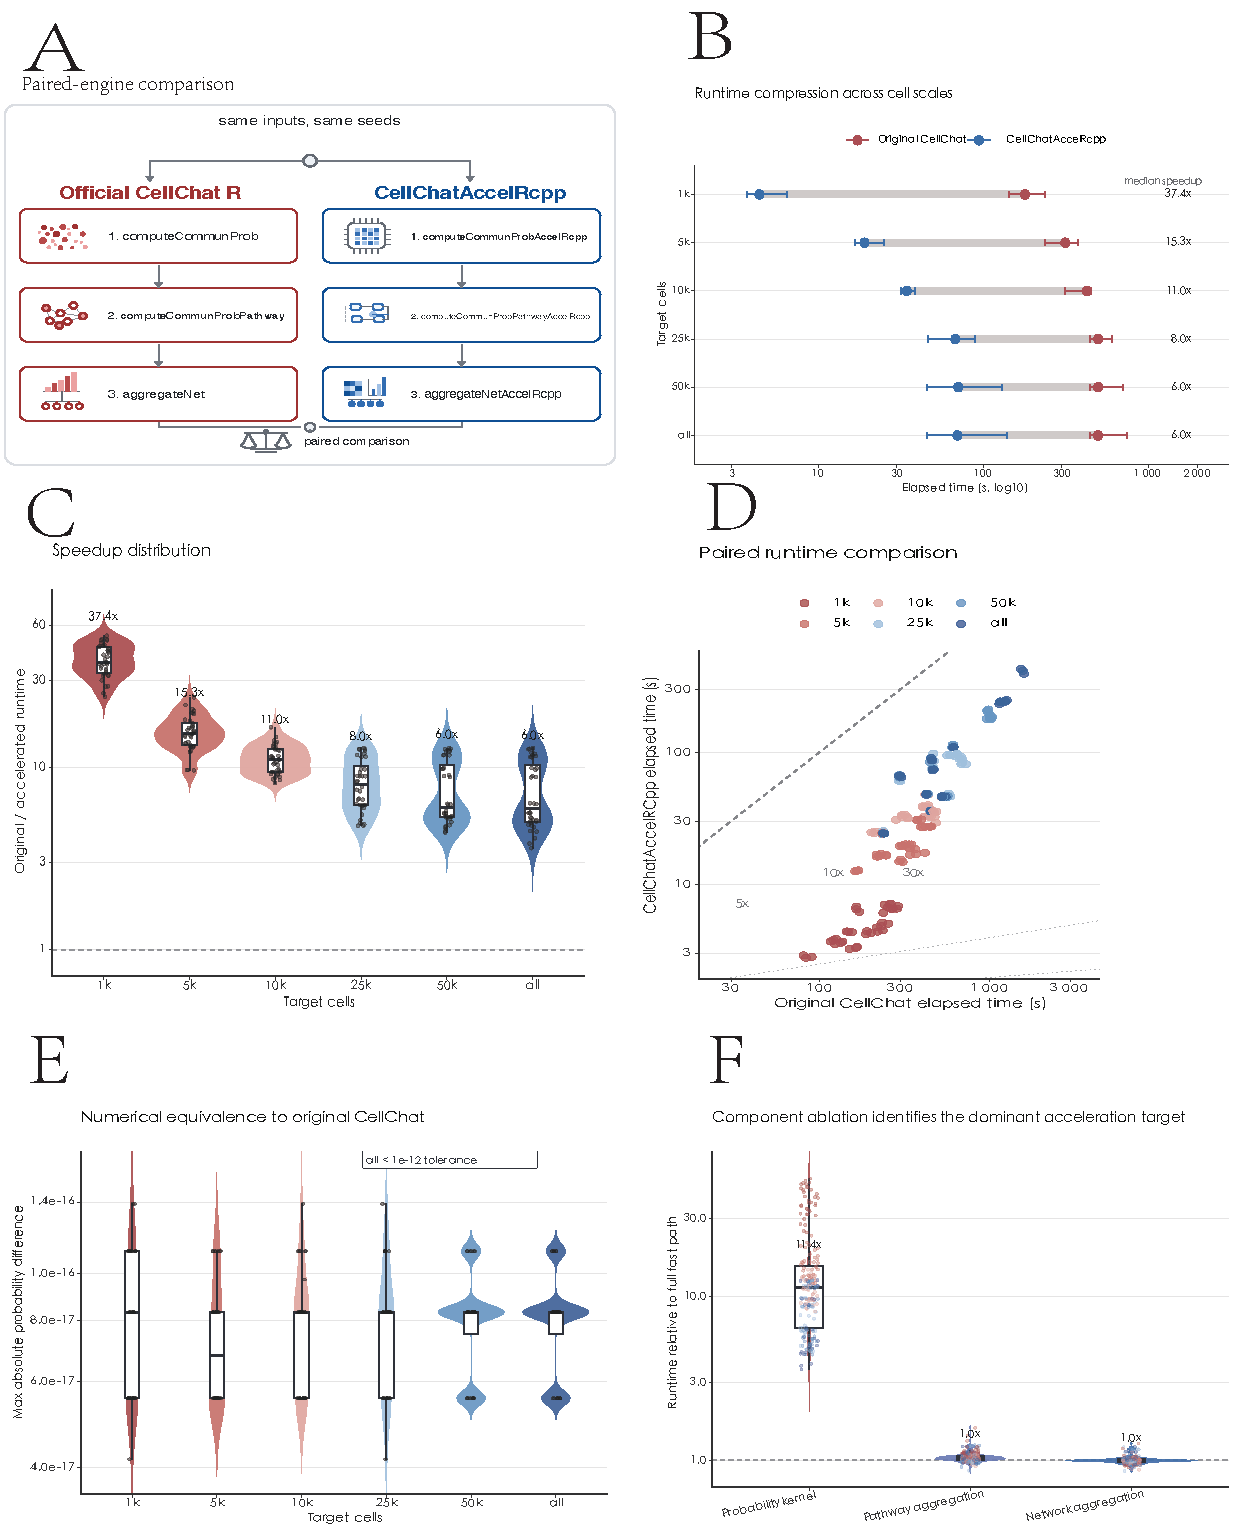
\includegraphics[width=0.93\textwidth]{1.pdf}
\figalttext[Six-panel performance summary for CellChatAccelRcpp]{Six-panel figure summarizing the CellChatAccelRcpp workflow, runtime compression, speedup distribution, paired runtime comparison, numerical agreement and component ablation results.}
\caption{
\textbf{CellChatAccelRcpp enables scalable and numerically matched CellChat inference.}
(A) Workflow overview of the accelerated CellChat pipeline.
(B) Runtime compression across target cell scales for original CellChat and CellChatAccelRcpp.
(C) Distribution of paired speedups, calculated as original CellChat runtime divided by accelerated runtime.
(D) Paired runtime comparison for matched dataset-scale-repeat experiments.
(E) Numerical equivalence between original and accelerated communication probability tensors, summarized by maximum absolute probability differences.
(F) Component ablation showing runtime changes when individual accelerated stages are disabled.
}
\label{fig:main}
\end{figure*}

\clearpage

\section{Availability and implementation}

CellChatAccelRcpp is available at \url{https://github.com/Blake-Deng/CellChatAccelRcpp} under the GPL-3 license.
The package depends on R ($\geq$ 4.1.0), Rcpp and an installed CellChat workflow.
The repository provides installation instructions, example usage, batch scripts, a conda environment file, equivalence checks, benchmark scripts, processed result tables, Supplementary Table S1 and figure-generation code.
The exact manuscript benchmark tables are stored under \url{benchmarks/cellchat_acceleration_2026/results/tables/}.

\section{Discussion}

CellChatAccelRcpp provides a pragmatic acceleration layer for large CellChat analyses.
By preserving the CellChat object interface and matching original probability tensors to floating-point precision, it supports larger single-cell cohorts without forcing users to change biological interpretation, plotting functions or downstream network summaries.
The strongest use cases are repeated subsampling studies, comparative analyses across many datasets, parameter checks and method-development workflows where the same CellChat inference is run many times.

The current scope is intentionally narrow.
CellChatAccelRcpp focuses on RNA-based, non-spatial, single-dataset CellChat workflows under the triMean setting.
Future development should broaden compatibility with additional CellChat options, spatial workflows and newer CellChat object structures.
The benchmark results nevertheless show that compiled acceleration of the dominant probability kernel is sufficient to make many large CellChat analyses substantially more tractable while preserving numerical agreement with the original implementation.

\section{Acknowledgements}

The author thanks the developers of CellChat, Rcpp and the open-source single-cell analysis ecosystem.
AI-assisted tools were used for language editing and manuscript preparation support; the author reviewed and is responsible for the analysis, interpretation and final manuscript content.

\section{Funding}

This work received no specific funding.

\section{Conflict of interest}

The author declares no competing interests.

\section{Data availability}

The benchmark datasets were derived from publicly available single-cell datasets.
Processed benchmark tables, figure-generation scripts and reproducibility instructions are available in the GitHub repository.
Dataset accession identifiers are listed in Supplementary Table S1.

\bibliographystyle{oup-plain}
\bibliography{references}

\end{document}
